\documentclass[aps,prl,reprint,nofootinbib,superscriptaddress]{revtex4-2}

\usepackage{graphicx}
\usepackage{hyperref}
\usepackage{amsmath, amssymb, amsthm}
\usepackage{booktabs}
\usepackage{siunitx}

\newtheorem{theorem}{Theorem}

%% Bundle: L1 (Tier 2; PRL splash; Phase 7b sub-wave 7b.0)
%% Generated 2026-05-01; lifted from paper25_gravitational_waves
%% (Phase 6a Wave 2). Schema: docs/BUNDLE_DIRECTORY_SCHEMA.md.
%% Source manifest: papers/L1/source_manifest.md.

\input{../../docs/counts.tex}

\newcommand{\cGW}{c_{\rm GW}}
\newcommand{\chivest}{\chi_{\rm vest}}
\newcommand{\dccap}{\Delta c/c}

\begin{document}

\title{GW170817 confines the vestigial-second-sound graviton
identification to one part in $10^{15}$ of its natural range}

\author{John G.\ Roehm}
\affiliation{NetRxn Foundation}

\date{\today}

\begin{abstract}
We constrain our assumed leading-order graviton speed
$\cGW=c\sqrt{\chivest}$, where $c$ is the electromagnetic
reference speed. The conservative GW170817 bound
$|\dccap|\leq\tau=3\times10^{-15}$ confines the nonnegative
susceptibility to $[(1-\tau)^2,(1+\tau)^2]$, of width $4\tau$.
This interval contains $\chivest=1$ and is over fourteen orders of
magnitude narrower than our adopted range $[0.1,10]$.
The mode and range are not derived from microscopic dynamics;
the constraint applies to this kinematic model, not to emergent
gravity generally.
\end{abstract}

\maketitle

%% ================================================================
\section{Introduction}
\label{sec:intro}

Spinor-gravity constructions use composite vielbeins built from
fermions~\cite{Diakonov2011,HebeckerWetterich2003}.
Volovik proposes a vestigial phase with metric order preceding a
nonzero tetrad expectation~\cite{Volovik2024Vestigial}.
His symmetry-breaking analysis distinguishes absorbed
Nambu--Goldstone modes from the Higgs-sector gravitational-wave
modes, whose counting also uses coordinate
constraints~\cite{Volovik2022Counting}.
Here we assume that a metric-channel excitation of such a substrate
can be identified with a spin-2 second-sound graviton.

\paragraph{Motivation and assumed speed law.}
Volovik applies Landau two-fluid hydrodynamics to a de~Sitter
state in~\cite{Volovik2026SecondSound}.
The underlying thermodynamic framework treats the gravitational
normal component as stiff matter~\cite{Volovik2024VacuumDecay}.
Within that de~Sitter model, the Landau formula and the stiff-component
thermodynamic relations give $s_2=c$, independently of $H$.
He discusses several possible graviton interpretations of this
collective mode and leaves its type open.
For the spin-2 substrate identification assumed here, we also assume
the susceptibility-dependent speed law:
\begin{equation}
  \cGW^2(\chivest) = c^2 \cdot \chivest, \qquad
  \cGW(\chivest) = c\sqrt{\chivest},
  \label{eq:cGW}
\end{equation}
where $\chivest$ is the dimensionless, normalized metric-channel
response of the assumed vestigial substrate.
It is a free parameter in this calculation.
The RPA form in \texttt{VestigialSusceptibility.lean} models it using
unevaluated bare susceptibility and coupling inputs, so that form
alone supplies no numerical value of $\chivest$.
The underlying
lattice-fermion framework is the one whose unitarity Vergeles
establishes~\cite{Vergeles2025}. Equation~\eqref{eq:cGW} is an
assumed kinematic speed law.
We constrain its free susceptibility without deriving a propagating
second-sound mode from a microscopic action, its propagator, or its
coupling to matter. This missing dynamical bridge is a limitation of
the present calculation, not an impossibility result.

The 2017 binary-neutron-star merger
GW170817~\cite{Abbott2017GW170817} yielded a tight propagation
constraint under the collaboration's conservative distance and
emission-time assumptions. Comparing the gravitational-wave arrival
time at LIGO/Virgo with the gamma-ray signal at Fermi/INTEGRAL gives
$-3 \times 10^{-15} \leq \dccap \leq +7 \times 10^{-16}$
under those assumptions. We use its conservative symmetric envelope,
$|\dccap| \leq \tau$ with $\tau = 3 \times 10^{-15}$.
This cap inherits the assumed source-emission window; alternative
emission histories can weaken the inferred propagation constraint.

Our assumed speed law satisfies the GW170817 bound only on a
sub-interval of our adopted range $\chivest \in [0.1, 10]$ narrower
than that range by more than 14 orders of magnitude. The
GW170817-compatible window $[(1-\tau)^2, (1+\tau)^2]$ has width
$4\tau$ in $\chivest$ and sits strictly interior to our adopted range
$[0.1, 10]$ about the anchor $\chivest = 1$.
Its relative width is $4\tau/9.9 \approx 1.2\times10^{-15}$;
a probability mass additionally requires a specified prior. The result is a fine-tuning constraint on one specific
kinematic identification, not a refutation of emergent
gravity nor of the ADW program; we discuss three Phase~6 recovery
paths in the Discussion.

\paragraph{Relation to the 2017 constraint sweep.} Using GW170817 to
eliminate a gravity model is not new. Within months of the detection,
four Letters analyzed constraints on specified gravitational actions
and cosmological models. Baker \emph{et al.}~\cite{BakerBellini2017}
constrained scalar-tensor and vector-tensor theories and obtained a
conditional graviton-mass bound in bimetric gravity. Creminelli and
Vernizzi~\cite{CreminelliVernizzi2017} required luminal propagation
to remain robust on nearby cosmological backgrounds to avoid tuning,
reducing the three independent quartic and quintic beyond-Horndeski
functions to one. Sakstein and Jain~\cite{SaksteinJain2017} combined
the GW bound with cluster and stellar tests to constrain
beyond-Horndeski parameters; their separate combination of GW and M87
black-hole constraints made the covariant quartic galileon
cosmologically irrelevant for the order-unity matter couplings
considered. Ezquiaga and
Zumalac\'arregui~\cite{EzquiagaZumalacarregui2017} also discussed
constraints on GW-speed-modifying couplings in Einstein-aether,
some sectors of Ho\v{r}ava gravity, and Generalized Proca theories,
and the impact on TeVeS and MOND-like theories.

These four analyses relate GW propagation to specified actions or EFT
operators, with assumptions about backgrounds and matter coupling.
They restrict combinations of functions or couplings, mass parameters,
and model cosmologies. This Letter supplies no microscopic Lagrangian for the
vestigial-second-sound identification. As the Introduction notes,
$\cGW = c\sqrt{\chivest}$ is assumed kinematically, so this calculation
does not constrain microscopic operator coefficients.
What the bound constrains is $\chivest$: the compatible interval has
roughly one part in $10^{15}$ of the width of our adopted order-unity
window. This is an interval-width comparison, not a microscopic
prediction of $\chivest$ or a probability statement independent of a prior. The
2017 sweep constrained \emph{theories}; this constrains an
\emph{identification}, which is why it is stated as a ratio of two
interval widths rather than as a surviving region of parameter space.

At fixed assumed Eq.~\eqref{eq:cGW}, this calculation constrains
$\chivest$ rather than microscopic operator coefficients. It does not
analyze whether the operator-level mechanisms discussed in those
theories alter the effective speed law or its applicability. A
microscopic realization would require that separate analysis.
The three recovery paths in
the Discussion can supply a mechanism fixing $\chivest$
within the compatible interval, or modify the identification or its
leading-order assumptions. A fixed-point mechanism can preserve the
speed law; the finite-tolerance constraint alone derives none of
these mechanisms.

%% ================================================================
\section{Formal setup and result}
\label{sec:result}

\paragraph{Vestigial-susceptibility natural range.}
Our substrate models the vestigial-phase metric-channel susceptibility
by the RPA \emph{resummation}
$\chi_{\rm RPA} = \chi_0/(1 - \gamma_\star \chi_0)$ in the standard
Hertz--Millis convention. Here $\chi_0$ is the bubble integral;
$\chi_{\rm RPA}$ is the resummed response and $\gamma_\star$ the
effective coupling; physical normalization remains undetermined.
\texttt{VestigialSusceptibility.lean} formalizes that closed form and
its stability properties; it evaluates neither $\chi_0$ nor
$\gamma_\star$, so it fixes no numerical $\chivest$, which is why
$\chivest$ enters Eq.~\eqref{eq:cGW} as a free parameter. The natural range
$\chivest \in [0.1, 10]$
is a \emph{project-adopted} naturalness window: the one-loop bubble
normalization is $\mathcal{O}(\Lambda_{\rm UV}^2/16\pi^2)$ by
dimensional analysis, and we take the $\pm 1$-decade window about
the resulting unit-normalized central value. We emphasize the
provenance: the window is a modeling choice of this project, not a
published derivation: the Vergeles lattice
analysis~\cite{Vergeles2025} establishes unitarity of the underlying
Einstein--Cartan--Palatini lattice theory but does not itself
compute $\chivest$ or assign it a range. The window matches the
linearized-EFE wave's ADW microscopic-coefficient
$\alpha_{\rm ADW} \in [0.1, 10]$ natural
range~\cite{Roehm2026LinearizedEFE}, which we treat as the
project-internal anchor for the order-of-magnitude prior.

\paragraph{The leading-order $\cGW$.}
Under the assumed law~\eqref{eq:cGW}, a positive susceptibility
and physical reference speed $c>0$ give $\cGW>0$.
For every $c\ne0$, the relative speed deviation is
\[
  \dccap(\chivest)
  \equiv \frac{\cGW(\chivest)-c}{c}
  = \sqrt{\chivest}-1.
\]
On the nonnegative domain this deviation is strictly increasing
and vanishes if and only if $\chivest=1$. Thus unity is the exactly
luminal anchor; finite-tolerance compatibility requires an interval
rather than this single value.

\paragraph{Finite-tolerance compatibility.}
Fix $\tau=3\times10^{-15}$ and write
$\verb|LigoSatisfied|(\delta)\equiv|\delta|\leq\tau$
for the conservative symmetric cap.

\begin{theorem}[\texttt{c\_GW\_match\_iff\_chi\_close\_to\_one}]
  \label{thm:bicond}
  For $\chivest\geq0$,
  $\verb|LigoSatisfied|(\dccap(\chivest))
  \;\Longleftrightarrow\;
  \chivest\in[(1-\tau)^2,(1+\tau)^2]$.
\end{theorem}

Indeed, the cap is equivalent to
$1-\tau\leq\sqrt{\chivest}\leq1+\tau$.
Since $0<\tau<1$, both bounds are nonnegative, so squaring
gives the stated interval. Conversely, monotonicity of the
square root recovers the cap from these squared bounds.

Every compatible susceptibility therefore satisfies
\[
  0.1<(1-\tau)^2\leq\chivest\leq(1+\tau)^2<10.
\]
The compatible interval contains $\chivest=1$ and has nonzero width exactly
$(1+\tau)^2-(1-\tau)^2=4\tau=1.2\times10^{-14}$.
The adopted range has width $9.9$, and the strict comparison is
\[
  10^{14}\bigl[(1+\tau)^2-(1-\tau)^2\bigr]<9.9.
\]
This is a comparison of interval widths within an adopted domain.
It supplies no probability without a prior: under a uniform prior
on $[0.1,10]$, the compatible interval has probability mass
$4\tau/9.9$.

\paragraph{Endpoint checks.}
The endpoints provide quantitative checks of the confinement.

\begin{theorem}[\texttt{natural\_lower\_violates\_ligo}]
  \label{thm:falsifier-lower}
  At $\chivest=0.1$, $\dccap=\sqrt{0.1}-1\approx-0.6838$,
  hence $|\dccap|/\tau\approx2.28\times10^{14}$ and
  \verb|LigoSatisfied| is false.
\end{theorem}

\begin{theorem}[\texttt{natural\_upper\_violates\_ligo}]
  \label{thm:falsifier-upper}
  At $\chivest=10$, $\dccap=\sqrt{10}-1\approx+2.1623$,
  hence $|\dccap|/\tau\approx7.21\times10^{14}$ and
  \verb|LigoSatisfied| is false.
\end{theorem}

The exclusions already follow from
$\sqrt{1/10}\leq\sqrt{1/4}=1/2$ and
$\sqrt{10}\geq\sqrt{4}=2$.
Both endpoints therefore fail simultaneously, while the finite
interval in Theorem~\ref{thm:bicond} remains compatible.
Figure~\ref{fig:cGW} shows this distinction.

\begin{figure}[t]
  \centering
  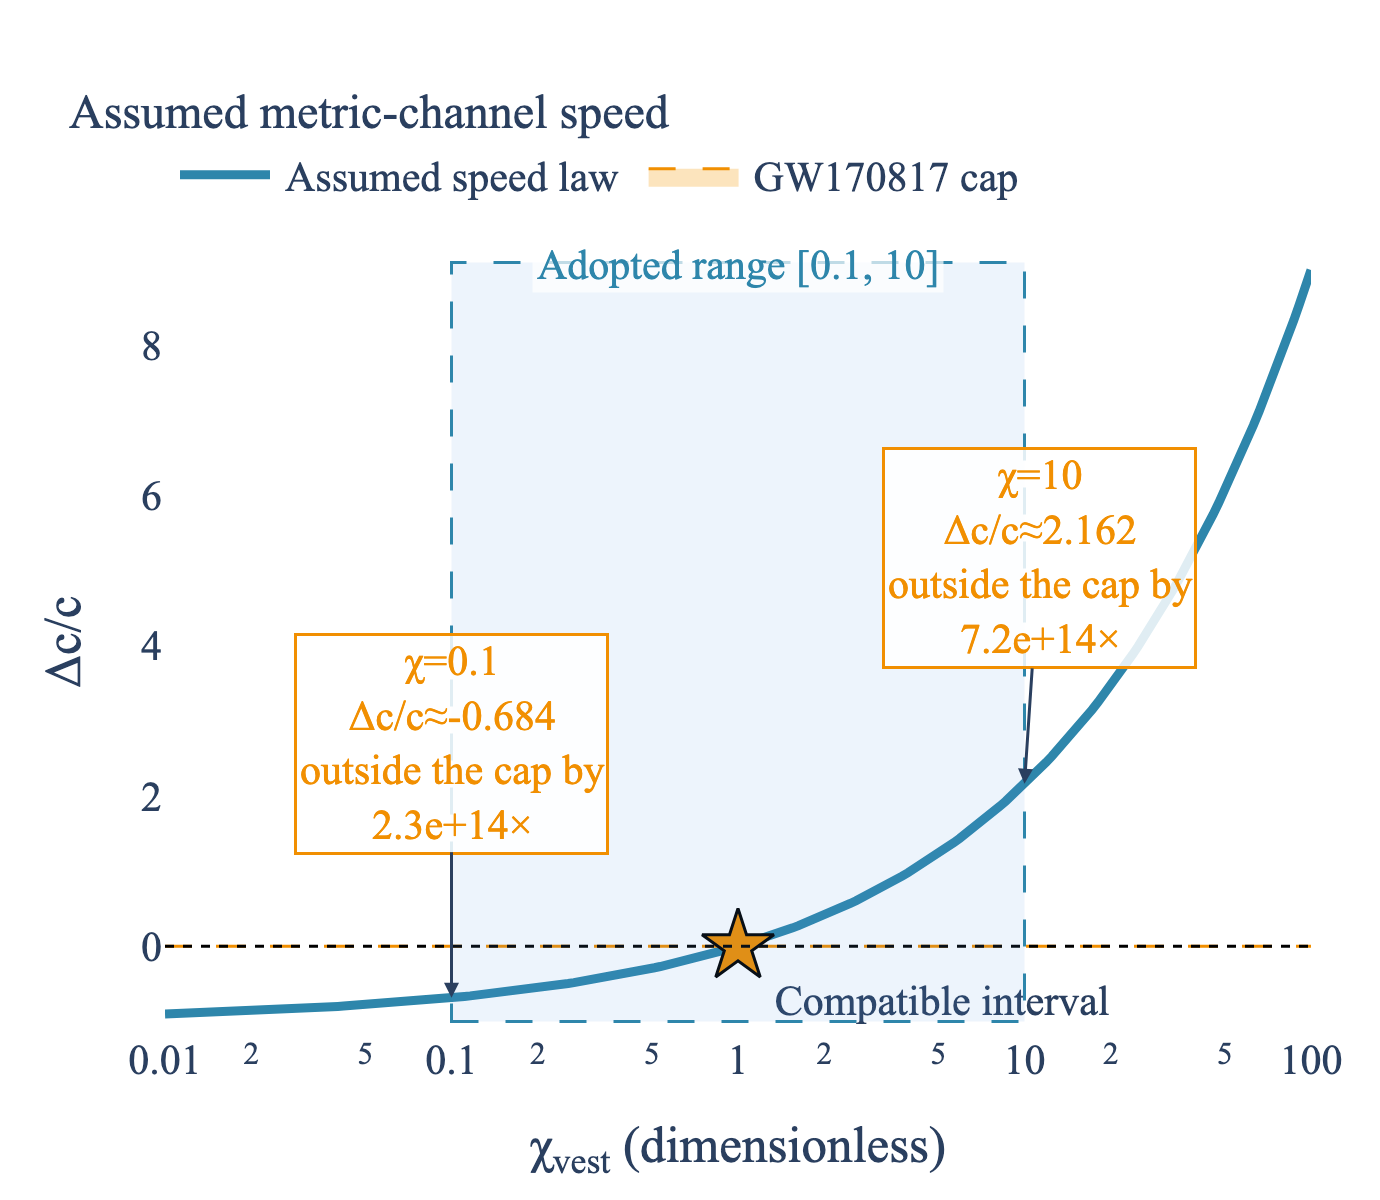
\includegraphics[width=0.96\columnwidth]{figures/fig_c_GW_vs_ligo_constraint.png}
  \caption{\textbf{Headline result.} The
  $\dccap = \sqrt{\chivest} - 1$ deviation across the natural
  $\chivest \in [0.1,10]$ range (pale blue band, dashed blue border)
  versus the conservative symmetric envelope of the
  GW170817~\cite{Abbott2017GW170817} multi-messenger constraint,
  $|\dccap| \leq 3\times 10^{-15}$ (amber, drawn at $\dccap = 0$ because
  the cap's own width is far below one pixel at this scale). Over the
  natural range $\dccap$ sweeps $[-0.68, +2.16]$, exceeding the cap by
  $\sim 10^{14}\times$ \emph{at the endpoints} (orange callouts) and
  vanishing at $\chivest = 1$. The compatible $\chivest$ window
  $[(1-\tau)^2,(1+\tau)^2]$ has width $4\tau = 1.2\times10^{-14}$,
  compared with the adopted range's width $9.9$. Its finite extent is
  unresolved at this scale; the gold star marks its anchor $\chivest=1$,
  not a singleton compatible set. The window sits \emph{inside} the band:
  the datum confines $\chivest$, it does not exclude the range.}
  \label{fig:cGW}
\end{figure}

\paragraph{Compatibility of the identification conditions.}
The proposed identification imposes positivity (P1), compatibility
with the cap (P2), and sub-half-deviation (P3'):
\[
  \begin{aligned}
    &\verb|H_VestigialModeIsGraviton|(\chivest)\\
    &\quad\equiv
      \chivest>0
      \;\wedge\;\verb|LigoSatisfied|(\dccap(\chivest))\\
    &\qquad\wedge\;|\dccap(\chivest)|<1/2.
  \end{aligned}
\]
These three clauses are not independent.
At the fixed tolerance, P2 implies P3' because $\tau<1/2$.
On the nonnegative domain, Theorem~\ref{thm:bicond} also places
every P2-compatible susceptibility in a strictly positive interval,
so P1 holds there. Consequently, the complete compatible set for
these conditions is precisely that same finite interval, including
the anchor $\chivest=1$.

Four counterexamples distinguish compatibility from positivity
alone. The endpoints $0.1$ and $10$ refute the conjunction through
failure of P2. At zero, P1 fails; this point lies outside the
adopted range. At the interior point $\chivest=1/4$,
$\dccap=-1/2$: P1 holds, but P2 and the strict P3' inequality
both fail. The quarter-point example therefore shows that P1
alone does not imply P3'. These counterexamples do not establish
independence of the three clauses or isolate a uniquely failing
clause. The corresponding definitions and algebraic results are
recorded in \texttt{GravitationalWaves.lean}, Sections~1--4.

\paragraph{Endpoint constraints and the open dynamical bridge.}
The endpoint exclusion also applies directly to the relative
deviation of the speed itself:
\[
  \left|\frac{\cGW(\chivest)-c}{c}\right|>\tau,
  \qquad
  \chivest\in\{0.1,10\},\quad c\ne0.
\]
This is the statement of
\texttt{natural\_endpoints\_violate\_ligo\_for\_every\_c};
it includes the physical domain $c>0$ and follows from the
relative-deviation identity above. Changing $c$ therefore
cannot make either endpoint compatible under the assumed law.
This two-point exclusion leaves the compatible interior interval
intact. Neither it nor the $c$-free endpoint statement quantifies
over microscopic actions, propagators or matter couplings, so
neither establishes the absence or impossibility of a dynamical
derivation. A physical application still requires the response
normalization and domain, the physical state, a propagating
tensor mode relative to the same matter/light reference, and
controlled transport and frequency matching with units and
error bounds.

%% ================================================================
\section{Discussion}
\label{sec:discussion}

\paragraph{What this constrains.} The conservative symmetric cap
restricts the assumed leading-order identification to
$\chivest\in[(1-\tau)^2,(1+\tau)^2]$.
Expanding the endpoints gives $1-2\tau+\tau^2$ and
$1+2\tau+\tau^2$: the susceptibility offsets are approximately
$\pm6\times10^{-15}$, whereas the speed-deviation tolerance is
$\pm3\times10^{-15}$. Exact luminality occurs at $\chivest=1$,
but the finite measurement tolerance permits a nonzero-width
interval. Its small relative width within our adopted range does not
alone establish a prior probability, rule out generic UV theories,
or require an exact fixed point at unity.

\paragraph{What this does not rule out.} Three Phase~6 paths remain
open:
\begin{enumerate}
\item \textbf{Symmetry-driven $\chivest \to 1$ fixed point.} If a
deep-IR symmetry (e.g.\ Lorentz invariance of the emergent metric
sector) makes $\chivest = 1$ an exact fixed point of the RG flow, the
fine-tuning is structural rather than tuned. An exact fixed point at $\chivest=1$ would lie inside the compatible
interval. The finite-tolerance constraint alone does not select this
mechanism or establish that a microscopic model realizes it.
Phase~6 should examine whether such a fixed point is realized in the
ADW broken phase.
\item \textbf{Distinct metric-channel identification.} We propose as an
alternative that the ``vestigial mode'' is a separate UV-input metric
channel rather than the second-sound DOF.
Its dynamics could in principle pin its susceptibility to unity;
this remains a model-building possibility. The missing dynamical
bridge in this Letter does not establish that this alternative is
more likely. Phase~6e (full nonlinear emergent action) is the natural
venue for the disambiguation.
\item \textbf{Frequency-dependent $\chivest$.} Equation~\eqref{eq:cGW} is
an assumed frequency-independent kinematic law.
A frequency-dependent susceptibility or a compensating correction
in the LIGO band is a possible phenomenological extension.
We consider the algebraic ansatz $\delta_{\rm disp}=\gamma\omega$,
without asserting that it is the leading term of a matched
microscopic derivative expansion.
The formal probe is numerical $\omega=100$; interpreting it as a
$100\,\mathrm{Hz}$ band and setting $\gamma=\Gamma_H/\cGW^2$ are
modeling assumptions requiring physical normalization and
microscopic matching.
\path{vestigial_dispersion_below_ligo_at_inspiral_peak}
assumes $|\gamma|\leq10^{-30}$ and proves that
$|\delta_{\rm disp}|$ at that numerical probe is below the
GW170817 tolerance.
The adopted $10^{-30}$ is a placeholder chosen to keep the
correction below the cap; it is neither derived nor measured.
In the further additive model
$\delta_{\rm tot}=\delta_0+\delta_{\rm disp}$, with
$\delta_0=\sqrt{\chivest}-1$, that assumed coefficient bound gives
$|\delta_{\rm disp}|\leq B=10^{-28}$ at $\omega=100$.
The reverse triangle inequality then excludes restoration of
$|\delta_{\rm tot}|\leq\tau$ whenever $|\delta_0|>\tau+B$.
Offsets just outside $\pm\tau$ can nevertheless become compatible
through an oppositely signed correction within this bound.
Larger corrections are not excluded by the placeholder theorem.
For a positive numerical probe $\omega$,
\texttt{dispersion\_within\_ligo\_iff} gives
$|\gamma\omega|\leq\tau\iff|\gamma|\leq\tau/\omega$ at the fixed
GW170817 tolerance $\tau$, bounding the correction alone.
\texttt{dispersion\_correction\_abs\_bound},
\texttt{dispersion\_correction\_linear\_in\_gamma} and
\path{dispersion_correction_zero_at_no_dissipation} describe
the product's magnitude, additivity in $\gamma$ and zero-coefficient
limit.
Deriving $\Gamma_H$ and the normalization of this ansatz from
microscopic dynamics remains open.
\end{enumerate}

\paragraph{Comparison to the linearized-EFE wave.} The companion
linearized-EFE wave~\cite{Roehm2026LinearizedEFE} ships an
emergent-gravity identification \emph{compatible} with observation at
the natural-range level: the Sakharov--Adler form
$G_{\rm N,emerg} = \alpha_{\rm ADW} \cdot 12\pi/(N_f \Lambda_{\rm UV}^2)$
at $\Lambda_{\rm UV} = M_{\rm Pl}$ produces
$\alpha_{\rm ADW}^\star \in [0.40, 1.27]$ for SM $N_f$, sitting
inside the natural range $[0.1,10]$. The asymmetry between the two
waves is a feature of the program: the linearized-EFE
$G_{\rm N,emerg}$ depends on the Sakharov--Adler kernel computed at
the linearized level, where the relevant scale is $M_{\rm Pl}$;
$\cGW$ depends on the free metric-channel susceptibility
$\chivest$. Our adopted interval contains unity but derives no
value of this susceptibility. The conservative GW170817 cap
restricts it to the much narrower compatible interval; the
width comparison alone supplies no microscopic selection mechanism.

\paragraph{Reproducibility.} The result is reproducible in two
layers. The Lean layer is \texttt{GravitationalWaves.lean} (32
theorems, zero \texttt{sorry}, zero new axioms, zero
\texttt{maxHeartbeats} overrides) at the project's pinned
Mathlib4 commit; the Python layer is \texttt{src/gravitational\_waves/}
with 89 \texttt{pytest} cases cross-checking every numeric quoted
in the abstract and figure caption. The headline figure
(\path{src/core/visualizations.py:fig_c_GW_vs_ligo_constraint})
and its underlying numerics are committed-pinned.

%% ================================================================
\begin{thebibliography}{99}

\bibitem{Volovik2024Vestigial}
G.~E.~Volovik, ``Fermionic Quartet and Vestigial Gravity,''
JETP Lett.\ \textbf{119}, 330 (2024);
DOI: 10.1134/S002136402460006X.

\bibitem{Volovik2022Counting}
G.~E.~Volovik, ``Gravity from Symmetry Breaking Phase Transition,''
J.~Low Temp.\ Phys.\ \textbf{207}, 127 (2022);
DOI: 10.1007/s10909-022-02694-z.

\bibitem{Volovik2026SecondSound}
G.~E.~Volovik, ``Massless graviton in de Sitter as second sound in
two-fluid hydrodynamics,'' arXiv:2601.00639v1 (2026).
\emph{Derives luminal second sound within its de~Sitter two-fluid
model and discusses possible graviton interpretations.}

\bibitem{Volovik2024VacuumDecay}
G.~E.~Volovik, ``From Landau two-fluid model to de Sitter Universe,''
arXiv:2410.04392v11 (2025).

\bibitem{Akama1978}
K.~Akama, Prog.\ Theor.\ Phys.\ \textbf{60}, 1900 (1978);
DOI: 10.1143/PTP.60.1900.

\bibitem{Diakonov2011}
D.~Diakonov, ``Towards lattice-regularized quantum gravity'',
arXiv:1109.0091 (2011).

\bibitem{VladimirovDiakonov2012}
A.~A.~Vladimirov and D.~Diakonov,
Phys.\ Rev.\ D \textbf{86}, 104019 (2012);
DOI: 10.1103/PhysRevD.86.104019.

\bibitem{HebeckerWetterich2003}
A.~Hebecker and C.~Wetterich,
Phys.\ Lett.\ B \textbf{574}, 269 (2003);
DOI: 10.1016/j.physletb.2003.09.010.

\bibitem{Wetterich2022}
C.~Wetterich, JHEP \textbf{06}, 069 (2022);
DOI: 10.1007/JHEP06(2022)069.

\bibitem{Vergeles2025}
S.~N.~Vergeles, Phys.\ Rev.\ D \textbf{112}, 054509 (2025);
DOI: 10.1103/PhysRevD.112.054509.

\bibitem{Abbott2017GW170817}
B.~P.~Abbott \emph{et al.}\ (LIGO/Virgo, Fermi GBM, INTEGRAL),
Astrophys.\ J.\ Lett.\ \textbf{848}, L13 (2017);
DOI: 10.3847/2041-8213/aa920c.

\bibitem{BakerBellini2017}
T.~Baker, E.~Bellini, P.~G.~Ferreira, M.~Lagos, J.~Noller and I.~Sawicki,
Phys.\ Rev.\ Lett.\ \textbf{119}, 251301 (2017);
DOI: 10.1103/PhysRevLett.119.251301.

\bibitem{CreminelliVernizzi2017}
P.~Creminelli and F.~Vernizzi,
Phys.\ Rev.\ Lett.\ \textbf{119}, 251302 (2017);
DOI: 10.1103/PhysRevLett.119.251302.

\bibitem{SaksteinJain2017}
J.~Sakstein and B.~Jain,
Phys.\ Rev.\ Lett.\ \textbf{119}, 251303 (2017);
DOI: 10.1103/PhysRevLett.119.251303.

\bibitem{EzquiagaZumalacarregui2017}
J.~M.~Ezquiaga and M.~Zumalac\'arregui,
Phys.\ Rev.\ Lett.\ \textbf{119}, 251304 (2017);
DOI: 10.1103/PhysRevLett.119.251304.

\bibitem{Roehm2026LinearizedEFE}
J.~G.~Roehm, ``Linearized Einstein Equations from
Anderson--Higgs Tetrad Condensation'',
\emph{SK--EFT-Hawking project, in preparation}, 2026
(\texttt{papers/paper23\_linearized\_efe/}).

\end{thebibliography}


%% ─── Lifted from _phase6o_W1b_lean_only (§4) — 2026-05-06T15:42:03Z ───
%% \section{G4 Kerr-Schild double-copy on Petrov-D analog gravity}
%% \label{sec:l1-_phase6o_W1b_lean_only}

%% Insertion point hint from PAPER_DRAFT_MAPPING.md: §4
%% Lift notes: D.2 absorption: Phase 6o W1b Kerr-Schild single-copy as alternative substrate context to vestigial graviton; cross-ref-only
%% NOTE: absorption DECLINED 2026-05-06; see papers/L1/append_log.json. The
%% three work markers formerly here were vestigial bookkeeping from that
%% abandoned lift, not outstanding work on L1, and were removed 2026-08-14
%% (review:2026-08-14-l1-stage13:L1:7.1). Had the lift proceeded it would
%% have owed: content from papers/_phase6o_W1b_lean_only/paper_draft.tex,
%% numerical claims traced via formulas.py / counts.tex, and primary-source
%% cache entries for its citations.

%% (Section heading + label commented out 2026-05-06 Session 2: empty post-bibliography stub from bundle_append.py default-insertion; bookkeeping anchor preserved as LaTeX comment, no rendered content. Append-log entry retains source-contribution registration.)
%% ─── End lift from _phase6o_W1b_lean_only ───

\end{document}
